\section{CLink\-Failed\-Exception  Class Reference}
\label{classCLinkFailedException}\index{CLinkFailedException@{CLink\-Failed\-Exception}}
{\tt \#include $<$CLink\-Failed\-Exception.h$>$}

Inheritance diagram for CLink\-Failed\-Exception::\begin{figure}[H]
\begin{center}
\leavevmode
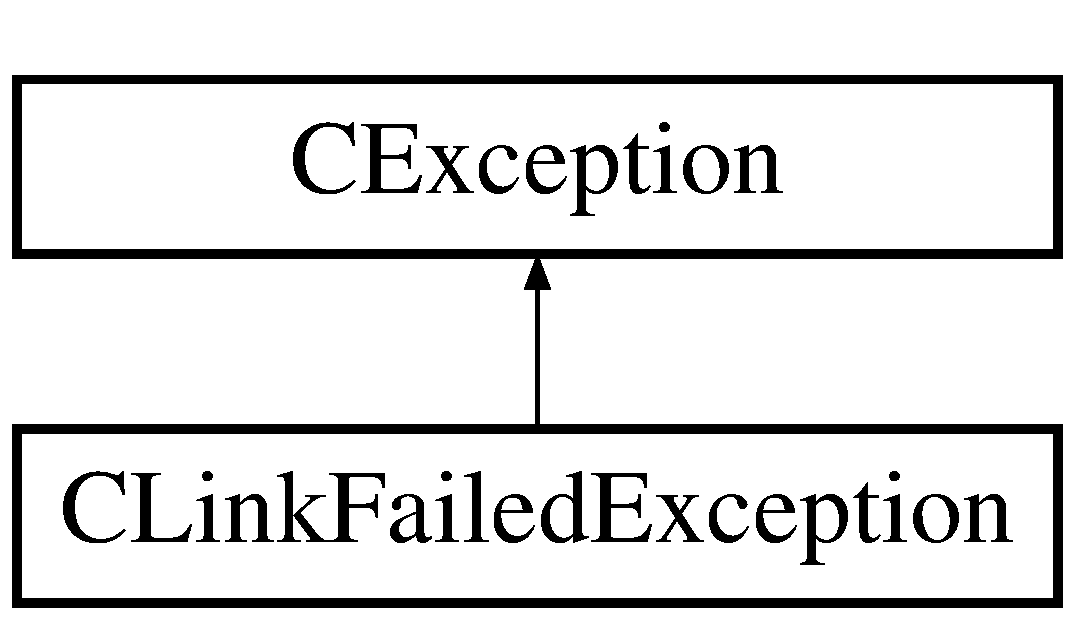
\includegraphics[height=2cm]{classCLinkFailedException}
\end{center}
\end{figure}
\subsection*{Public Methods}
\begin{CompactItemize}
\item 
{\bf CLink\-Failed\-Exception} (const char $\ast$p\-Doing, const char $\ast$p\-Name)
\item 
{\bf CLink\-Failed\-Exception} (const char $\ast$p\-Doing, const string \&r\-Name)
\item 
{\bf CLink\-Failed\-Exception} (const string \&r\-Doing, const char $\ast$p\-Name)
\item 
{\bf CLink\-Failed\-Exception} (const string \&r\-Doing, const string \&r\-Name)
\item 
{\bf CLink\-Failed\-Exception} (const string \&r\-Doing, int n\-Id)
\item 
{\bf CLink\-Failed\-Exception} (const char $\ast$p\-Doing, int n\-Id)
\item 
virtual {\bf $\sim$CLink\-Failed\-Exception} ()
\item 
{\bf CLink\-Failed\-Exception} (const CLink\-Failed\-Exception \&a\-CLink\-Failed\-Exception)
\item 
CLink\-Failed\-Exception {\bf operator=} (const CLink\-Failed\-Exception \&a\-CLink\-Failed\-Exception)
\item 
int {\bf operator==} (const CLink\-Failed\-Exception \&a\-CLink\-Failed\-Exception)
\item 
string {\bf get\-Name} () const
\item 
void {\bf set\-Name} (string am\_\-s\-Name)
\item 
virtual const char $\ast$ {\bf Reason\-Text} () const
\end{CompactItemize}
\subsection*{Protected Methods}
\begin{CompactItemize}
\item 
void {\bf Update\-Reason\-Text} ()
\end{CompactItemize}
\subsection*{Private Attributes}
\begin{CompactItemize}
\item 
string {\bf m\_\-s\-Name}
\item 
int {\bf m\_\-n\-Id}
\item 
bool {\bf m\_\-f\-Name}
\item 
string {\bf m\_\-s\-Reason\-Text}
\end{CompactItemize}


\subsection{Constructor \& Destructor Documentation}
\index{CLinkFailedException@{CLink\-Failed\-Exception}!CLinkFailedException@{CLinkFailedException}}
\index{CLinkFailedException@{CLinkFailedException}!CLinkFailedException@{CLink\-Failed\-Exception}}
\subsubsection{\setlength{\rightskip}{0pt plus 5cm}CLink\-Failed\-Exception::CLink\-Failed\-Exception (const char $\ast$ {\em p\-Doing}, const char $\ast$ {\em p\-Name})\hspace{0.3cm}{\tt  [inline]}}\label{classCLinkFailedException_a0}




Definition at line 301 of file CLink\-Failed\-Exception.h.

References m\_\-f\-Name, m\_\-s\-Name, and Update\-Reason\-Text().\index{CLinkFailedException@{CLink\-Failed\-Exception}!CLinkFailedException@{CLinkFailedException}}
\index{CLinkFailedException@{CLinkFailedException}!CLinkFailedException@{CLink\-Failed\-Exception}}
\subsubsection{\setlength{\rightskip}{0pt plus 5cm}CLink\-Failed\-Exception::CLink\-Failed\-Exception (const char $\ast$ {\em p\-Doing}, const string \& {\em r\-Name})\hspace{0.3cm}{\tt  [inline]}}\label{classCLinkFailedException_a1}




Definition at line 307 of file CLink\-Failed\-Exception.h.

References m\_\-f\-Name, m\_\-s\-Name, and Update\-Reason\-Text().\index{CLinkFailedException@{CLink\-Failed\-Exception}!CLinkFailedException@{CLinkFailedException}}
\index{CLinkFailedException@{CLinkFailedException}!CLinkFailedException@{CLink\-Failed\-Exception}}
\subsubsection{\setlength{\rightskip}{0pt plus 5cm}CLink\-Failed\-Exception::CLink\-Failed\-Exception (const string \& {\em r\-Doing}, const char $\ast$ {\em p\-Name})\hspace{0.3cm}{\tt  [inline]}}\label{classCLinkFailedException_a2}




Definition at line 313 of file CLink\-Failed\-Exception.h.

References m\_\-f\-Name, m\_\-s\-Name, and Update\-Reason\-Text().\index{CLinkFailedException@{CLink\-Failed\-Exception}!CLinkFailedException@{CLinkFailedException}}
\index{CLinkFailedException@{CLinkFailedException}!CLinkFailedException@{CLink\-Failed\-Exception}}
\subsubsection{\setlength{\rightskip}{0pt plus 5cm}CLink\-Failed\-Exception::CLink\-Failed\-Exception (const string \& {\em r\-Doing}, const string \& {\em r\-Name})\hspace{0.3cm}{\tt  [inline]}}\label{classCLinkFailedException_a3}




Definition at line 319 of file CLink\-Failed\-Exception.h.

References m\_\-f\-Name, m\_\-s\-Name, and Update\-Reason\-Text().\index{CLinkFailedException@{CLink\-Failed\-Exception}!CLinkFailedException@{CLinkFailedException}}
\index{CLinkFailedException@{CLinkFailedException}!CLinkFailedException@{CLink\-Failed\-Exception}}
\subsubsection{\setlength{\rightskip}{0pt plus 5cm}CLink\-Failed\-Exception::CLink\-Failed\-Exception (const string \& {\em r\-Doing}, int {\em n\-Id})\hspace{0.3cm}{\tt  [inline]}}\label{classCLinkFailedException_a4}




Definition at line 325 of file CLink\-Failed\-Exception.h.

References m\_\-f\-Name, m\_\-n\-Id, and Update\-Reason\-Text().\index{CLinkFailedException@{CLink\-Failed\-Exception}!CLinkFailedException@{CLinkFailedException}}
\index{CLinkFailedException@{CLinkFailedException}!CLinkFailedException@{CLink\-Failed\-Exception}}
\subsubsection{\setlength{\rightskip}{0pt plus 5cm}CLink\-Failed\-Exception::CLink\-Failed\-Exception (const char $\ast$ {\em p\-Doing}, int {\em n\-Id})\hspace{0.3cm}{\tt  [inline]}}\label{classCLinkFailedException_a5}




Definition at line 331 of file CLink\-Failed\-Exception.h.

References m\_\-f\-Name, m\_\-n\-Id, and Update\-Reason\-Text().\index{CLinkFailedException@{CLink\-Failed\-Exception}!~CLinkFailedException@{$\sim$CLinkFailedException}}
\index{~CLinkFailedException@{$\sim$CLinkFailedException}!CLinkFailedException@{CLink\-Failed\-Exception}}
\subsubsection{\setlength{\rightskip}{0pt plus 5cm}virtual CLink\-Failed\-Exception::$\sim$CLink\-Failed\-Exception ()\hspace{0.3cm}{\tt  [inline, virtual]}}\label{classCLinkFailedException_a6}




Definition at line 337 of file CLink\-Failed\-Exception.h.\index{CLinkFailedException@{CLink\-Failed\-Exception}!CLinkFailedException@{CLinkFailedException}}
\index{CLinkFailedException@{CLinkFailedException}!CLinkFailedException@{CLink\-Failed\-Exception}}
\subsubsection{\setlength{\rightskip}{0pt plus 5cm}CLink\-Failed\-Exception::CLink\-Failed\-Exception (const CLink\-Failed\-Exception \& {\em a\-CLink\-Failed\-Exception})\hspace{0.3cm}{\tt  [inline]}}\label{classCLinkFailedException_a7}




Definition at line 341 of file CLink\-Failed\-Exception.h.

References m\_\-s\-Name, and Update\-Reason\-Text().

\subsection{Member Function Documentation}
\index{CLinkFailedException@{CLink\-Failed\-Exception}!getName@{getName}}
\index{getName@{getName}!CLinkFailedException@{CLink\-Failed\-Exception}}
\subsubsection{\setlength{\rightskip}{0pt plus 5cm}string CLink\-Failed\-Exception::get\-Name () const\hspace{0.3cm}{\tt  [inline]}}\label{classCLinkFailedException_a10}




Definition at line 371 of file CLink\-Failed\-Exception.h.

References m\_\-s\-Name.\index{CLinkFailedException@{CLink\-Failed\-Exception}!operator=@{operator=}}
\index{operator=@{operator=}!CLinkFailedException@{CLink\-Failed\-Exception}}
\subsubsection{\setlength{\rightskip}{0pt plus 5cm}CLink\-Failed\-Exception CLink\-Failed\-Exception::operator= (const CLink\-Failed\-Exception \& {\em a\-CLink\-Failed\-Exception})\hspace{0.3cm}{\tt  [inline]}}\label{classCLinkFailedException_a8}




Definition at line 351 of file CLink\-Failed\-Exception.h.

References m\_\-s\-Name, CException::operator=(), and Update\-Reason\-Text().\index{CLinkFailedException@{CLink\-Failed\-Exception}!operator==@{operator==}}
\index{operator==@{operator==}!CLinkFailedException@{CLink\-Failed\-Exception}}
\subsubsection{\setlength{\rightskip}{0pt plus 5cm}int CLink\-Failed\-Exception::operator== (const CLink\-Failed\-Exception \& {\em a\-CLink\-Failed\-Exception})\hspace{0.3cm}{\tt  [inline]}}\label{classCLinkFailedException_a9}




Definition at line 362 of file CLink\-Failed\-Exception.h.

References m\_\-s\-Name, and CException::operator==().\index{CLinkFailedException@{CLink\-Failed\-Exception}!ReasonText@{ReasonText}}
\index{ReasonText@{ReasonText}!CLinkFailedException@{CLink\-Failed\-Exception}}
\subsubsection{\setlength{\rightskip}{0pt plus 5cm}const char $\ast$ CLink\-Failed\-Exception::Reason\-Text () const\hspace{0.3cm}{\tt  [virtual]}}\label{classCLinkFailedException_a12}


Returns a const pointer to text which describes the reason the exception was thrown. This is exception type specific. The default action returns a pointer to the constant string: \char`\"{}Unspecified Exception\char`\"{} 

Reimplemented from {\bf CException} {\rm (p.\,\pageref{classCException_a8})}.

Definition at line 285 of file CLink\-Failed\-Exception.cpp.

References m\_\-s\-Reason\-Text.\index{CLinkFailedException@{CLink\-Failed\-Exception}!setName@{setName}}
\index{setName@{setName}!CLinkFailedException@{CLink\-Failed\-Exception}}
\subsubsection{\setlength{\rightskip}{0pt plus 5cm}void CLink\-Failed\-Exception::set\-Name (string {\em am\_\-s\-Name})\hspace{0.3cm}{\tt  [inline]}}\label{classCLinkFailedException_a11}




Definition at line 377 of file CLink\-Failed\-Exception.h.

References m\_\-s\-Name.\index{CLinkFailedException@{CLink\-Failed\-Exception}!UpdateReasonText@{UpdateReasonText}}
\index{UpdateReasonText@{UpdateReasonText}!CLinkFailedException@{CLink\-Failed\-Exception}}
\subsubsection{\setlength{\rightskip}{0pt plus 5cm}void CLink\-Failed\-Exception::Update\-Reason\-Text ()\hspace{0.3cm}{\tt  [protected]}}\label{classCLinkFailedException_b0}




Definition at line 291 of file CLink\-Failed\-Exception.cpp.

References m\_\-n\-Id, m\_\-s\-Name, and m\_\-s\-Reason\-Text.

Referenced by CLink\-Failed\-Exception(), and operator=().

\subsection{Member Data Documentation}
\index{CLinkFailedException@{CLink\-Failed\-Exception}!m_fName@{m\_\-fName}}
\index{m_fName@{m\_\-fName}!CLinkFailedException@{CLink\-Failed\-Exception}}
\subsubsection{\setlength{\rightskip}{0pt plus 5cm}bool CLink\-Failed\-Exception::m\_\-f\-Name\hspace{0.3cm}{\tt  [private]}}\label{classCLinkFailedException_o2}




Definition at line 297 of file CLink\-Failed\-Exception.h.

Referenced by CLink\-Failed\-Exception().\index{CLinkFailedException@{CLink\-Failed\-Exception}!m_nId@{m\_\-nId}}
\index{m_nId@{m\_\-nId}!CLinkFailedException@{CLink\-Failed\-Exception}}
\subsubsection{\setlength{\rightskip}{0pt plus 5cm}int CLink\-Failed\-Exception::m\_\-n\-Id\hspace{0.3cm}{\tt  [private]}}\label{classCLinkFailedException_o1}




Definition at line 296 of file CLink\-Failed\-Exception.h.

Referenced by CLink\-Failed\-Exception(), and Update\-Reason\-Text().\index{CLinkFailedException@{CLink\-Failed\-Exception}!m_sName@{m\_\-sName}}
\index{m_sName@{m\_\-sName}!CLinkFailedException@{CLink\-Failed\-Exception}}
\subsubsection{\setlength{\rightskip}{0pt plus 5cm}string CLink\-Failed\-Exception::m\_\-s\-Name\hspace{0.3cm}{\tt  [private]}}\label{classCLinkFailedException_o0}




Definition at line 295 of file CLink\-Failed\-Exception.h.

Referenced by CLink\-Failed\-Exception(), get\-Name(), operator=(), operator==(), set\-Name(), and Update\-Reason\-Text().\index{CLinkFailedException@{CLink\-Failed\-Exception}!m_sReasonText@{m\_\-sReasonText}}
\index{m_sReasonText@{m\_\-sReasonText}!CLinkFailedException@{CLink\-Failed\-Exception}}
\subsubsection{\setlength{\rightskip}{0pt plus 5cm}string CLink\-Failed\-Exception::m\_\-s\-Reason\-Text\hspace{0.3cm}{\tt  [private]}}\label{classCLinkFailedException_o3}




Definition at line 298 of file CLink\-Failed\-Exception.h.

Referenced by Reason\-Text(), and Update\-Reason\-Text().

The documentation for this class was generated from the following files:\begin{CompactItemize}
\item 
{\bf CLink\-Failed\-Exception.h}\item 
{\bf CLink\-Failed\-Exception.cpp}\end{CompactItemize}
